
\section*{Introducción}
Los amplificadores operacionales (op-amps) son dispositivos electrónicos fundamentales en el diseño de circuitos analógicos, ya que permiten amplificar señales muy pequeñas, realizar operaciones matemáticas y procesar información en función a una configuración entre sus entradas, siendo así que para tal propósito es necesario contar con cierta precisión entre su terminales diferenciales, por lo tanto un análisis de las corrientes de polarización es necesario para lograr este objetivo el cual afecta a mediciones de rango pequeño como las provenientes del cuerpo humano o en la industrial en las cuales los requisitos de voltaje y/o corriente son pequeños para extender el tiempo de vida de un determinado sensor.

Así mismo dentro del desarrollo de esta experiencia se verá en pleno funcionamiento de 2 amplificadores operacionales y su respuesta y/o tensión de offset y corrientes de bias (polarización) entre sus entradas inversora y no inversora, para lo cual se emplea un circuito de prueba.


\section{ Mediciones de voltaje divisor de tensión y amplificadores operacionales}

Como punto de partida se compararon los niveles de voltaje obtenidos a partir de un divisor de tensión utilizando el mismo circuito en un etapa posterior para la medición del voltaje obtenido previamente mediante los operacionales LM741 y el TL081 en una configuración de seguidor de voltaje, en la figura \ref{fig:divisor-tension} la configuración inicial y en la figura \ref{fig:seguidor-tension} la configuración para los operacionales anteriormente mencionados.

\begin{figure}[h]
	\centering
	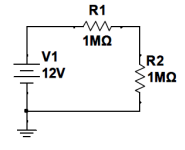
\includegraphics[width=0.3\linewidth]{media/divisor-tension}
	\caption{Medición de voltaje - divisor de tensión}
	\label{fig:divisor-tension}
\end{figure}

% TODO: \usepackage{graphicx} required
\begin{figure}[h]
	\centering
	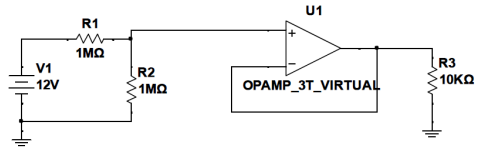
\includegraphics[width=0.8\linewidth]{media/seguidor-tension}
	\caption{Seguidor de tensión}
	\label{fig:seguidor-tension}
\end{figure}

Las mediciones para cada circuito con el operacional indicado se muestran en la tabla \ref{tab:mediciones-voltaje} y de la cual se puede inferir que existen una cierta variación entre los valores esperados idealmente según las consideraciones teóricas para los amplificadores operacionales, lo que destaca en cierta forma la existencia de un fenómeno electrico no considera dentro del análisis general usado para el estudio de los operacionales.

\begin{table}[]
	\begin{tabular}{|l|l|}
		\hline
		& Voltaje {[}V{]} \\ \hline
		R2    & 5.61            \\ \hline
		LM741 & 5.88            \\ \hline
		TL081 & 5.9             \\ \hline
	\end{tabular}
	\caption{Mediciones de voltaje}
	\label{tab:mediciones-voltaje}
\end{table}

\subsection{Voltaje medido y esperado}
Debido a las diferencias de voltaje para componente usado en la experiencia este de forma teórica se debido aproximar al voltaje medido en la resistencia $R_2$ y el cual se esperaba verse reflejado en la resistencia $R_3$, sin embargo y como se verá más adelante la diferencia entre estos valores de salida ocurre a un desbalance en la entrada de cada operacional y que se conoce como los valores offset el amp. operacional y que se debe tener en cuenta para aplicaciones que requieran de pequeñas variaciones en las salidas.

\section{Medición $V_O$ y cálculo de $V_{OS}$ }

Las mediciones realizadas durante la experiencia se realizaron en el circuito mostrado en la figura \ref{fig:opam-offset} y con el cual bajo las consideraciones indicadas $R_4$ y $R_5$ cortocircuitadas, se realizo la medición del voltaje de salida $V_O$ y en función a ello se determino el valor de $V_{OS}$ en función a la relación indicada en \ref{eq:vos-calculo}.

\begin{equation}
	V_{OS} = -\frac{V_O}{1 + \frac{R_6}{100}}
	\label{eq:vos-calculo}
\end{equation}

Obteniendo como medición y resultado para cada operacional los datos mostrados en la tabla \ref{tab:mediciones-vo-vos} denotándose una pequeña variación en las tensiones de salida que rondan tan solo las milésima y con un error \% de 0.00982. 

\begin{table}[]
	\begin{tabular}{|l|l|l|}
		\hline
		\multicolumn{1}{|c|}{\textbf{Dispositivo}} & \multicolumn{1}{c|}{\textbf{Vo}} & \multicolumn{1}{c|}{\textbf{Vos}} \\ \hline
		\textbf{LM741}                             & -10.173                          & 0.01016284                        \\ \hline
		\textbf{TL081}                             & -10.174                          & 0.01016384                        \\ \hline
	\end{tabular}
	\caption{Valores de $V_O$ y $V_{OS}$ - LM741, TL081}
	\label{tab:mediciones-vo-vos}
\end{table}

% TODO: \usepackage{graphicx} required
\begin{figure}[h]
	\centering
	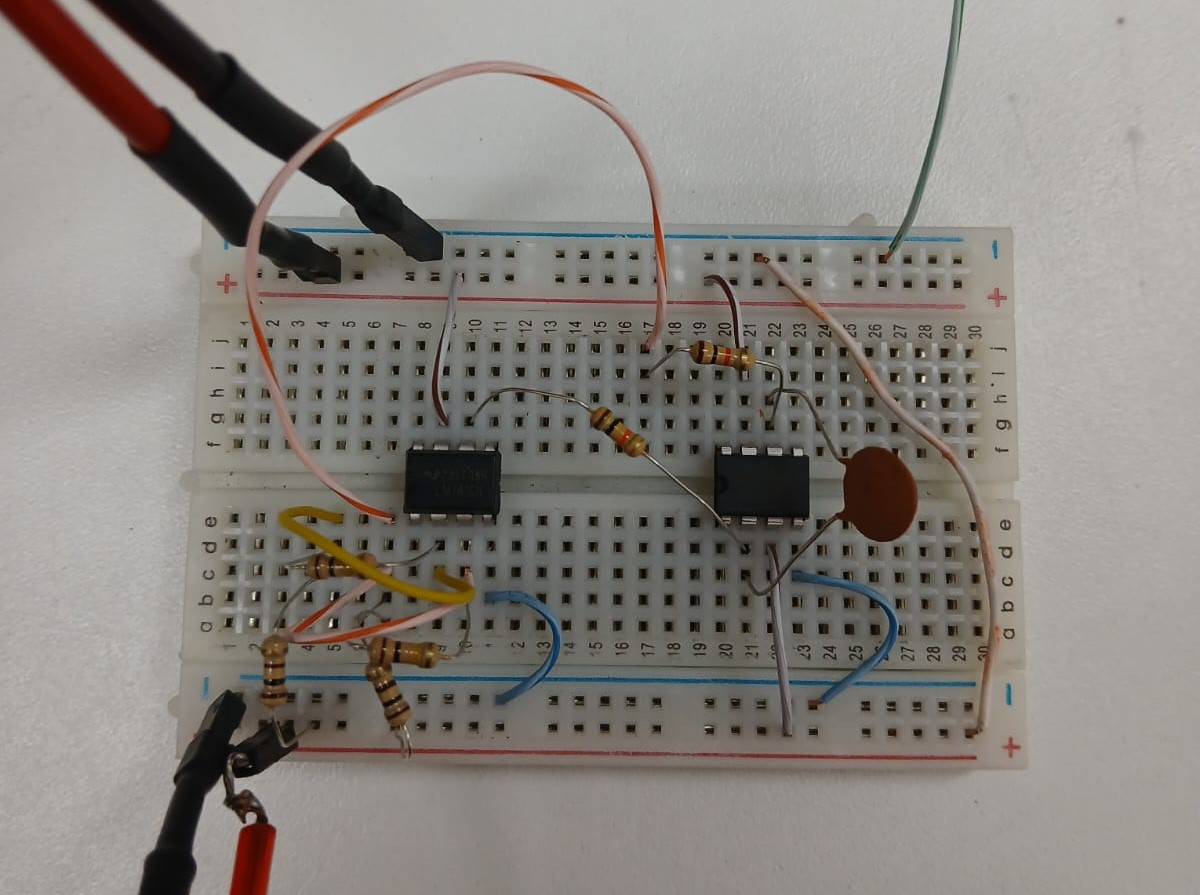
\includegraphics[width=0.5\linewidth]{media/opam-offset}
	\caption{Circuito de prueba para las mediciones offset en los amplificadores operacionales}
	\label{fig:opam-offset}
\end{figure}


\section{Resultados finales}


























